\documentclass[12pt, a4paper, oneside]{ctexart}
\usepackage{amsmath, amsthm, amssymb, graphicx}
\usepackage{float}
\usepackage{diagbox}
\usepackage[bookmarks=true, colorlinks, citecolor=blue, linkcolor=black]{hyperref}

% tikz画图包
\usepackage{pgfplots}
\usetikzlibrary{patterns,arrows,positioning,calc,fadings,shapes,decorations.markings}
\usepackage{tikz}

% 导言区
\title{作业二第6题}
\author{崔俊杰}

\begin{document}
\maketitle
\raggedright(1)电路的输出方程:\(Y = Q_2\) \\
\quad \\
\raggedright(2)电路的驱动方程:
$
\begin{cases}

    D_0 = Q_2^{'}Q_1^{'}Q_0^{'} \\
    D_1 = Q_0 \\
    D_2 = Q_1 

\end{cases}
$\\ 
\quad \\
\raggedright(3)电路的状态方程:\\
由D触发器的特性方程\(Q = D\)有\\
\begin{align}
    Q_0 &= J_1Q_1^{'} + K_1^{'}Q_1 \nonumber \\
    &= Q_3^{'}Q_1^{'} + Q_3Q_1 \nonumber \\
    &= Q_3 \odot Q_1 \nonumber
\end{align}
\begin{align}
    Q_2 &= J_2Q_2^{'} + K_2^{'}Q_2 \nonumber \\
    &= Q_2^{'}Q_1 + Q_2Q_1^{'} \nonumber \\
    &= Q_2 \oplus Q_1 \nonumber
\end{align}
\begin{align}
    Q_3 &= J_3Q_3^{'} + K_3^{'}Q_3 \nonumber \\
    &= Q_3^{'}Q_2Q_1 + Q_3^{'}Q_3 \nonumber \\
    &= Q_3^{'}Q_2Q_1 \nonumber
\end{align}
\raggedright 故电路的状态方程为:
$
\begin{cases}
    Q_1 = Q_3 \odot Q_1 \\ 
    Q_2 = Q_2 \oplus Q_1 \\ 
    Q_3 = Q_3^{'}Q_2Q_1 \\
\end{cases}
$\\
\; \\
\; \\
\raggedright(4)电路的状态图如图所示: \\
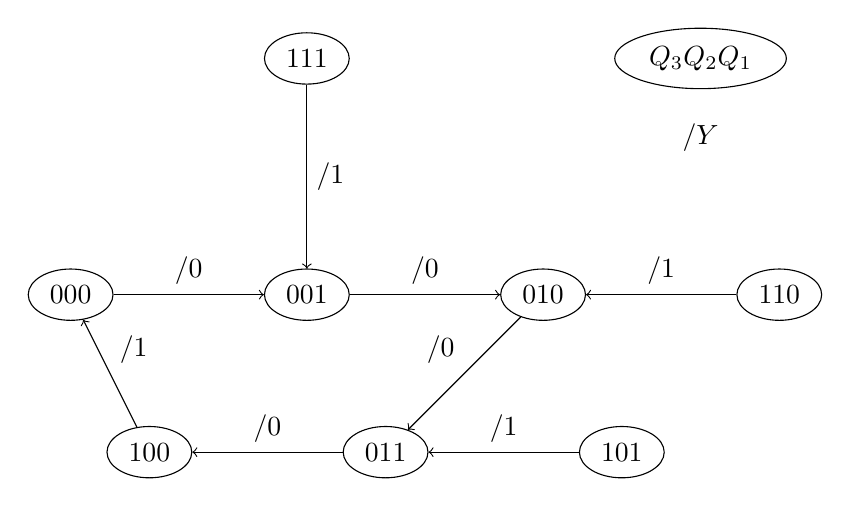
\begin{tikzpicture}
    \node (Y) at (10,0) {/$Y$};
    \node [draw,shape=ellipse](n1) at (2,-2) {000};
    \node [draw,shape=ellipse](n2) at (5,-2) {001};
    \node [draw,shape=ellipse](n3)at (8,-2) {010};
    \node [draw,shape=ellipse](n4)at (11,-2) {110};
    \node [draw,shape=ellipse](n5)at (3,-4) {100};
    \node [draw,shape=ellipse](n6)at (6,-4) {011};
    \node [draw,shape=ellipse](n7)at (9,-4) {101};
    \node [draw,shape=ellipse](n8)at (5,1) {111};
    \node [draw,shape=ellipse](n)at (10,1) {$Q_3Q_2Q_1$};

    \draw[->] (n1) -- node[above] {/0} (n2); 
    \draw[->] (n2) -- node[above] {/0} (n3); 
    \draw[->] (n4) -- node[above] {/1} (n3); 
    \draw[->] (n5) -- node[above right] {/1} (n1); 
    \draw[->] (n6) -- node[above] {/0} (n5); 
    \draw[->] (n7) -- node[above] {/1} (n6); 
    \draw[->] (n3) -- node[above left] {/0} (n6); 
    \draw[->] (n8) -- node[right] {/1} (n2);
\end{tikzpicture}
\\
\;\\
\textbf{由图可知,该电路可以自启动.} \\\;\\
\raggedright(5)分析电路的逻辑功能:\\
\textbf{由状态图可知,该电路实现的是一个时序模5计数器.}
\end{document}